\chapter{Introduction} \Contact{Alex}
\label{sec:intro}
\bigskip
\Contributors{Alex Drlica-Wagner, Keith Bechtol, Annika H.\ G.\ Peter, Yao-Yuan Mao}

The fundamental nature of dark matter, which constitutes $\roughly 85\%$ of the matter density and $\roughly 26\%$ of the energy density of the universe, represents a critical gap in our understanding of fundamental physics.
Over the past several decades, experimental searches for non-baryonic particle dark matter have proceeded along several complementary avenues (\figref{interactions}).
Collider experiments (\eg, ATLAS and CMS at the LHC) attempt to produce and detect dark matter particles, while  %\citep{Boveia:2018yeb,Ehret:2010mh,Battaglieri:2017aum}
direct detection experiments (\eg, LUX, LZ, XENON1T, SuperCDMS, ADMX, PICO, DAMiC, SENSEI, CRESST) attempt to directly detect energy deposition from very rare scattering between dark matter and Standard Model particles.
%\citep{1509:02910, 1804.10697, Du:2018uak} 
In parallel, indirect dark matter searches (\eg, {\it Fermi}-LAT, AMS-02, HESS, CTA, HAWC, {\it Chandra}, XMM) seek to detect the energetic Standard Model products from the annihilation or decay of dark matter particles {\it in situ} in astrophysical systems. %\citep[\eg][]{1503.02641,1402.2301, 1605.01043, 1603.06978}. 
Despite these extensive efforts, the only robust, positive empirical measurements of dark matter to date come from astrophysical and cosmological observations. 

Astrophysics and cosmology offer a complementary technique to study the fundamental properties of dark matter. 
They probe dark matter directly through gravity, the only force to which dark matter is known to couple. 
On large scales, observational data is well described by a simple model of stable, non-relativistic, collisionless, cold dark matter (CDM).
However, many viable theoretical models of dark matter predict observable deviations from CDM, which are testable with current and future experimental programs.
Fundamental properties of dark matter---e.g., particle mass, self-interaction cross section, coupling to the Standard Model, and time-evolution---can imprint themselves on the macroscopic distribution of dark matter in a detectable manner.

In addition, astrophysical observations complement particle physics searches by providing input to direct and indirect dark matter experiments, and by enabling alternative tests of dark matter's non-gravitational coupling to the Standard Model.  
For example, astrophysical observations can be used to i) measure the local distribution of dark matter, an important variable for direct searches, ii) highlight regions of high dark matter density for targeting indirect searches, and iii) identify astronomical objects that can lead to tight constraints on the range of dark matter particle mass and electric charge for a specific dark matter model.  
As the most widely studied CDM particle model, the weakly interacting massive particle (WIMP), becomes more and more tightly constrained, astrophysical observations will provide critical information to help direct future particle physics searches.  
In many cases, observations with telescopes provide \emph{the only} robust, empirical constraints on the viable range of dark matter models.

At the same time, there is immense dark matter discovery potential at the intersection of particle physics and astrophysics.
Detecting a deviation from the gravitational predictions of CDM would provide much-needed experimental guidance on parameters that are not easily measured in particle physics experiments (\eg, dark matter self-interaction cross sections). 
%If, on the other hand, all astrophysical studies of dark matter are found to agree with the CDM predictions, the improved knowledge of dark matter distributions will reduce major sources of theoretical uncertainties in the particle physics experiments. 
%ADW: I don't know what is being referred to here.
Likewise, results from particle experiments can suggest specific deviations from the CDM paradigm that can be tested with astrophysical observations.
The expanding landscape of theoretical models for dark matter provides strong motivation to explore dark matter parameter space beyond the current sensitivity of the high-energy physics program.

The Large Synoptic Survey Telescope (LSST) is a next-generation wide-area optical survey instrument that will probe the fundamental physics of dark matter and dark energy with precise cosmological measurements \citep{0805.2366,2018RPPh...81f6901Z}. 
Following on predecessors such as the Sloan Digital Sky Survey (SDSS) and the Dark Energy Survey (DES), LSST promises to greatly enhance our knowledge of the dark sector of the universe. 
LSST will measure the properties of dark matter over a wide range of astrophysical scales, thereby testing a wide variety of particle physics models (\tabref{models}).
At the largest scales, LSST will use gravitational weak lensing and the large-scale clustering of galaxies to trace the distribution of dark matter.
The profiles of dark matter halos associated with galaxies and clusters of galaxies can be used to test self-interacting dark matter models.
Measurements of the small-scale clustering of dark matter, traced by the faintest galaxies and via gravitational perturbations in strong lenses and stellar tracers, will enable constraints on warm and ultra-light dark matter models.
In addition, the temporal component of the LSST ``wide, fast, deep'' survey will open a new window on the search for compact dark matter, such as primordial black holes (PBHs).
LSST will provide a rich scientific data set that can be used to develop novel and unanticipated constraints on dark matter properties through precise measurements of physical processes, such as anomalous energy loss in stars that could be produced by axion-like particles.

In this white paper, we present several techniques that LSST will employ to probe the fundamental properties of dark matter. 
In \secref{theory} we discuss several theoretical models of dark matter that can be constrained by LSST.
In \secref{probes} we present several observational probes of novel dark matter physics, and the  measurements that LSST will make to access these probes.
Many astrophysical measurements require collaborative observations between several instruments, and the study of dark matter with LSST is no exception. 
Thus, in \secref{complementarity}, we discuss situations where LSST will complement other astrophysical and particle investigations of dark matter.
Finally, in \secref{discovery} we present two scenarios of dark matter discovery with LSST.
Rather than presenting a comprehensive review of astrophysical probes of dark matter  \citep[e.g.,][]{BuckleyPeter:2017} or an extensive discussion of any particular dark matter model \citep[e.g.,][]{Tulin:2017ara}, we choose to focus on what we believe are some of the most exciting opportunities to study dark matter physics with LSST. 
Our goal is to demonstrate that LSST will not only provide exciting results on the nature of dark matter, but that observations from LSST are {\it critical} to guide future particle physics searches.

\begin{figure}[t]
\centering
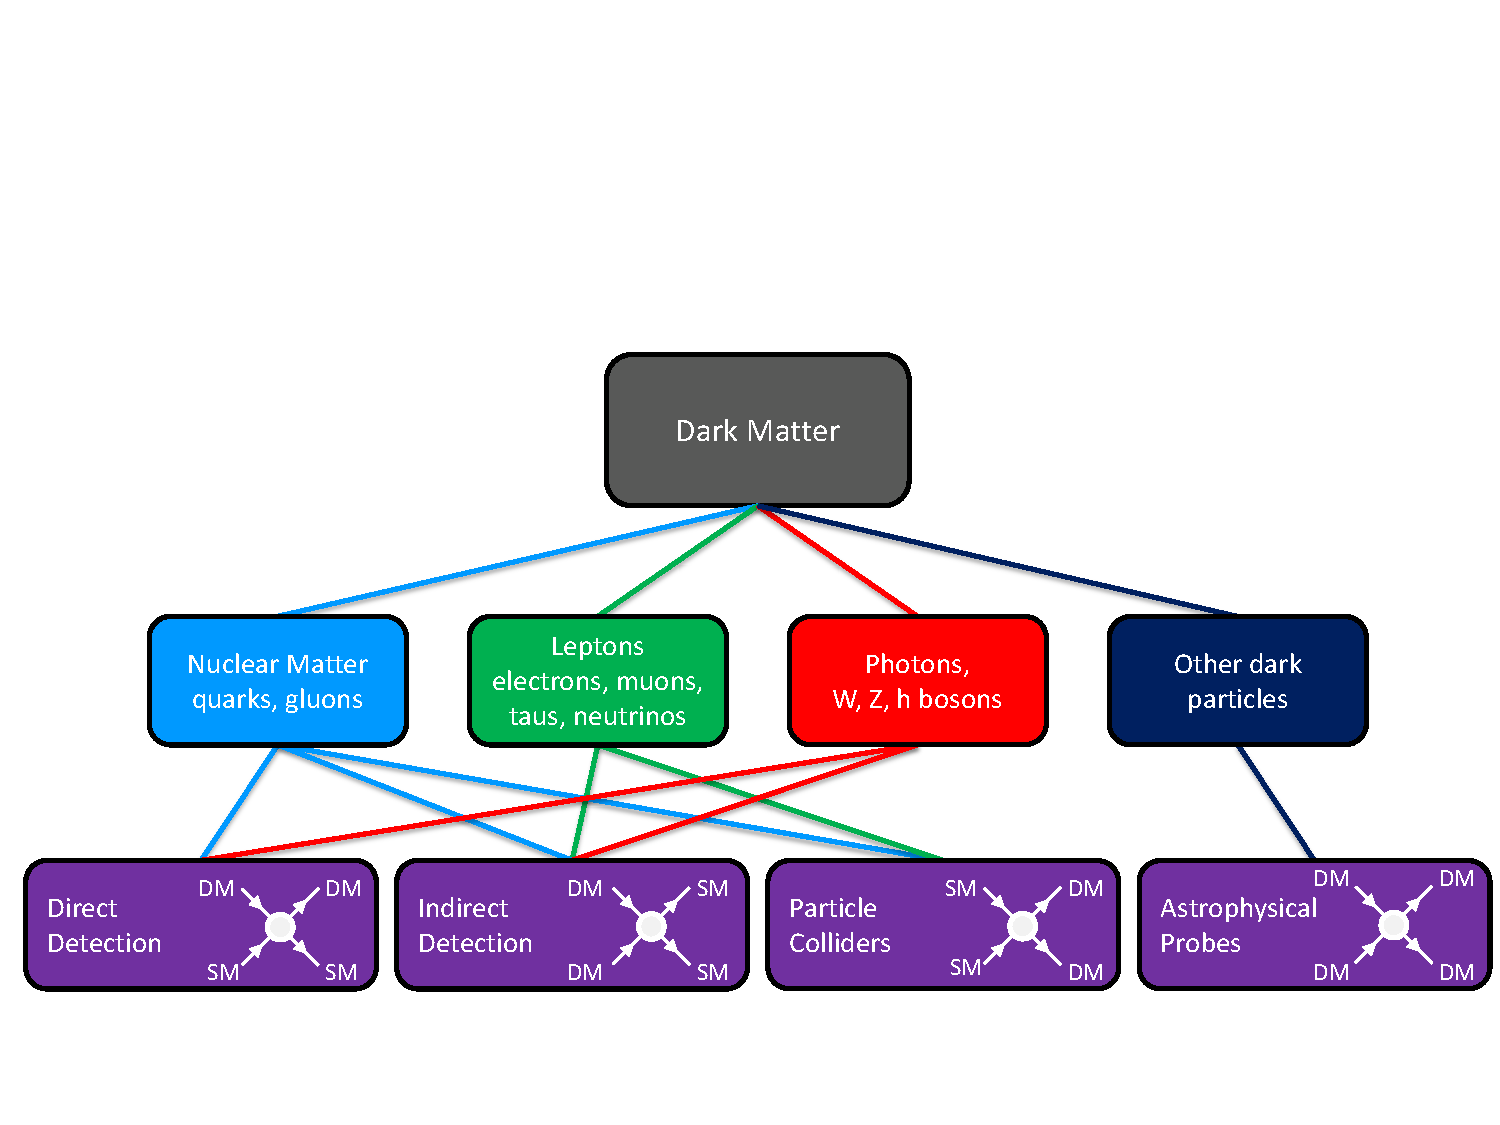
\includegraphics[width=0.85\textwidth]{figures/interactions.pdf}
\vspace{0.5em}
\caption{
\label{fig:interactions}
Dark matter may have non-gravitational interactions, which can be probed by four complementary approaches: 
direct detection, indirect detection, particle colliders, and astrophysical probes.
The lines connect the experimental approaches with the categories of particles that they most stringently probe (additional lines can be drawn in specific model scenarios). 
Figure taken from the Snowmass CF4 Report \citep{1305.1605}.
}
\end{figure}

\begin{table}[t]
\begin{center}
\begin{tabular}{l c c c}
\hline 
Model & Probe & Parameter & Value \\
\hline 
\hline
Warm Dark Matter  & Halo Mass & Particle Mass & \CHECK{$m \sim 18 \keV$} \\
Self-Interacting Dark Matter & Halo Profile & Cross Section & \CHECK{$\sigmam \sim 0.1\text{--}10\cm^2/\g$} \\
Baryon-Scattering Dark Matter & Halo Mass & Cross Section & \CHECK{$\sigma \sim 10^{-30} \cm^2$} \\
Axion-Like Particles & Energy Loss & Coupling Strength & \CHECK{$g_{\phi e} \sim 10^{-13} $} \\
Fuzzy Dark Matter & Halo Mass & Particle Mass & \CHECK{$m \sim 10^{-20} \eV$}  \\
Primordial Black Holes  & Compact Objects & Object Mass & \CHECK{$M > 10^{-4} \Msun$} \\
Weakly Interacting Massive Particles & Indirect Detection & Cross Section & \CHECK{$\sigmav \sim 10^{-27} \cm^3/\second$} \\
Light Relics & Large-Scale Structure & Relativistic Species & \CHECK{$N_{\rm eff} \sim 0.1$} \\[+0.5em]
\hline
\end{tabular}
\end{center}
\caption{\label{tab:models} Probes of fundamental dark matter physics with LSST. Classes of dark matter models are listed in Column 1, and the primary observational probe that is sensitive to each model is listed in Column 2. The corresponding dark matter parameters are listed in Column 3, and estimates of LSST's senstivity to each parameter are listed in Column 4.}
\end{table}

